% !TeX spellcheck = es_ES
% Chapter 1

%\chapter{Chapter Title Here} % Main chapter title
%
%\label{Chapter1} % For referencing the chapter elsewhere, use \ref{Chapter1} 

%----------------------------------------------------------------------------------------

% Define some commands to keep the formatting separated from the content 
%\newcommand{\tabhead}[1]{\textbf{#1}}
%\newcommand{\code}[1]{\texttt{#1}}
%\newcommand{\file}[1]{\texttt{\bfseries#1}}
%\newcommand{\option}[1]{\texttt{\itshape#1}}

%----------------------------------------------------------------------------------------

\chapter{Control de la temperatura}\label{ch: thermal}
	El sistema cuenta con dos calentadores de precisión al interior del baño termostatado de 25 litros. Estos calentadores junto con el ba\~no externo determinan la temperatura de trabajo del equipo. El ba\~no externo se usa con el objetivo de mantener siempre activos los calentadores internos en alg\'un nivel de potencia intermedio, pues el ba\~no externo, al tener una temperatura inferior agregar una carga permanente a los calentadores internos \cite{Suurkuusk}. Para monitorear la temperatura del ba\~no el calor\'imetro cuenta con dos termistores, el primero para trabajar a temperaturas inferiores a 50 \grad{} y el segundo para temperaturas superiores a este valor. La se\~nal generada por uno de estos termistores se compara con un valor de resistencia definido por el usuario. La resistencia y por ende la temperatura del equipo se fijan usando cuatro resistencias de década, esto es que cada resistencia es una potencia de 10 menor que la anterior, las cuales se encuentran en la parte inferior del calor\'imetro, en la \autoref{fig: decadeResistors} corresponden A, B, C, y D, de esta manera se pueden realizar experimentos a temperaturas en el rango de 5 a 80 \grad{}. El diagrama del sistema de control t\'ermico del calor\'imetro se muestra en el \autoref{anx: imagenes} como \autoref{fig: controlTermico}.
	
	\begin{figure}[h]
		\centering
		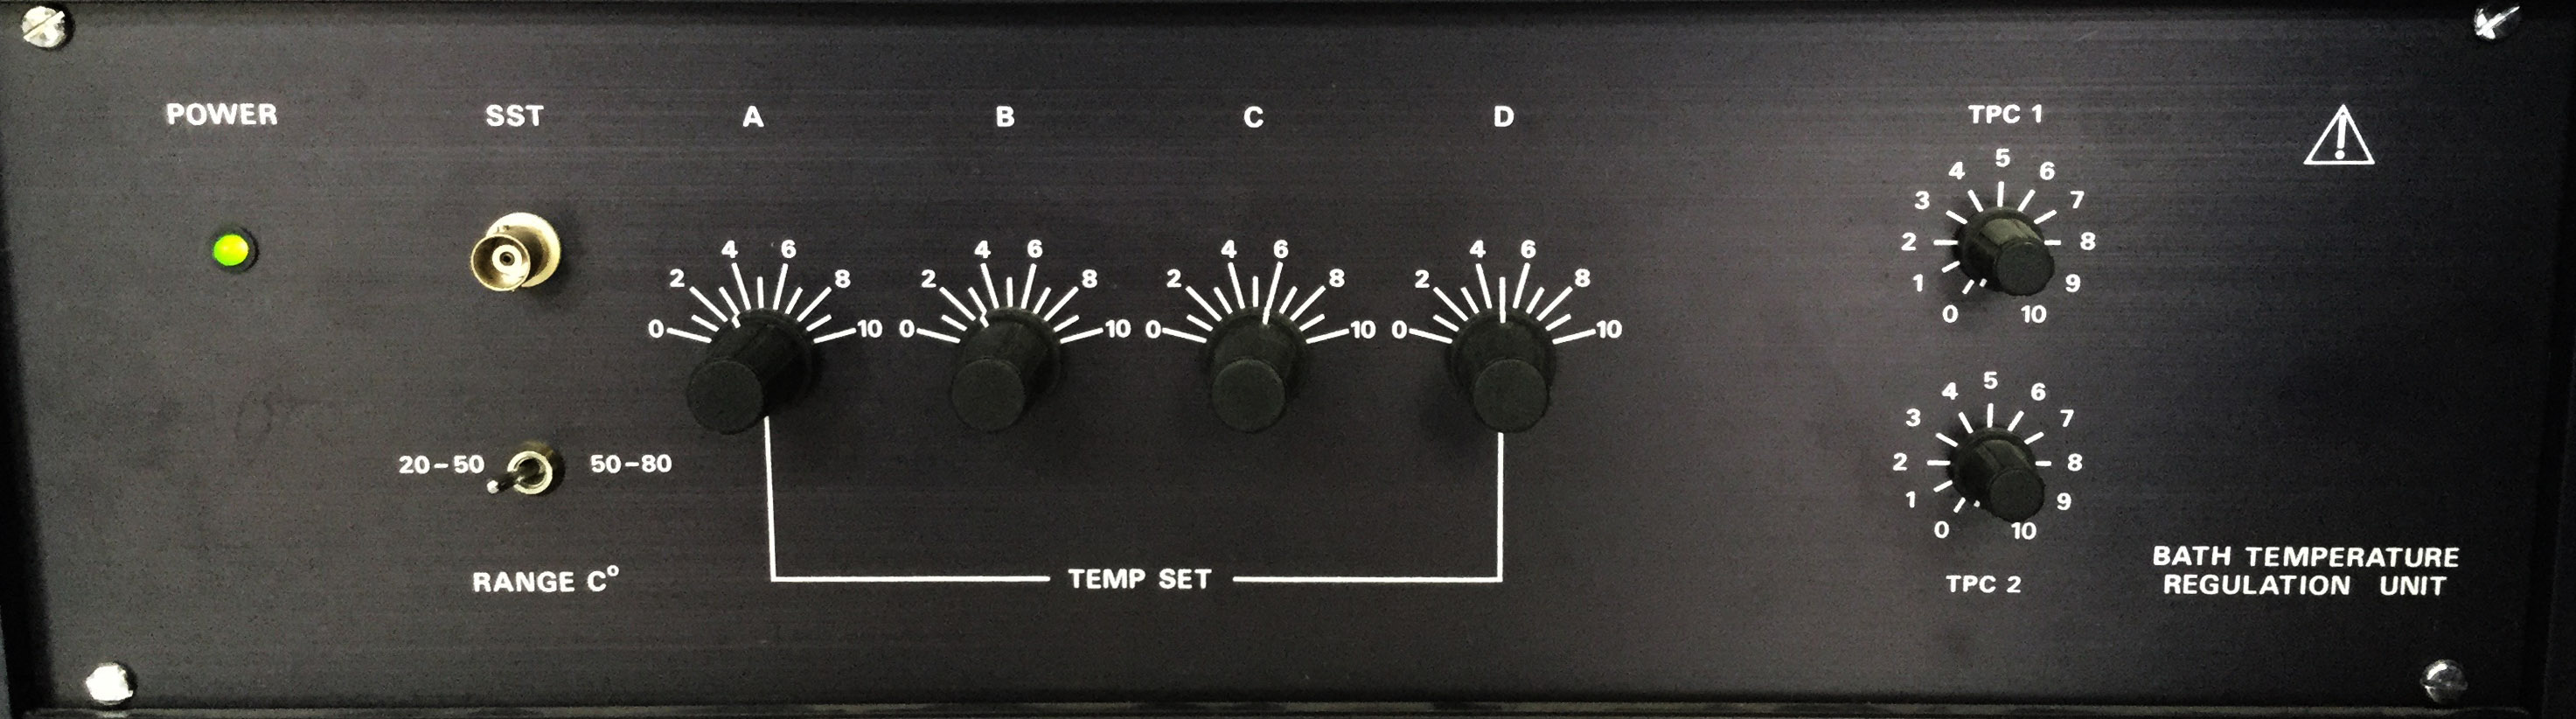
\includegraphics[width=0.7\linewidth]{Figures/decadeResistors}
		\caption{Resistencias de década que controlan la temperatura.}
		\label{fig: decadeResistors}
	\end{figure}
	
	Para determinar la equivalencia de resistencia y temperatura el calorímetro cuenta con una tabla que relaciona los valores de resistencia y temperatura de ba\~no externo que dan lugar a una temperatura constante en el ba\~no interno. Dicha tabla se muestra en el \autoref{ch: imagenes} como \autoref{fig: temperatureTable}, sin embargo, el uso de esa tabla est\'a limitado a temperaturas ambiente superiores a 20 \grad{} por lo cual, en el caso particular de Bogot\'a rara vez se cumplen. Lo anterior es relevante dado que la resistencia el\'ectrica depende de la temperatura, en el caso de materiales met\'alicos, la resistencia aumenta con la temperatura, y para semiconductores se tiene el efecto contrario \cite{simon2013oxford}.
	
	Una vez realizadas las conexiones el\'ectricas del calor\'imetro para su funcionamiento a 110 VAC, y antes de realizar una calibraci\'on qu\'imica fue necesario estabilizar el equipo a una temperatura de 25 \grad{}, puesto que el objetivo de la calibraci\'on qu\'imica es contrastar los datos obtenidos con el calor\'imetro con los reportados en la literatura, los cuales por convenci\'on se reportan a estas condiciones. Para alcanzar esta temperatura se probó con las condiciones reportadas en la \autoref{fig: temperatureTable}, en donde los valores de cada resistencia de década se muestra a continuación. 
	\begin{table}[h]
		\centering
		\caption{Valores de las resistencias de década, para una temperatura de 25 \grad{}, seg\'un calibración original del calorímetro.}
		\begin{tabular}{r|cccc|l}
			\hline
			\textbf{Baño interno (\grad{})} & A ($10^4$ $\Omega$) & B ($10^3$ $\Omega$) & C ($10^2$ $\Omega$) & D ($10^1$ $\Omega$) & \textbf{Baño externo (\grad{})} \\
			\hline
			25,0 & 3 & 2 & 4 & 9 & 22,0 \\
			\hline
		\end{tabular}
		\label{tb: decadeResistorsBefore}
	\end{table}
	
	La temperatura del equipo fue monitoreada por cuatro días, con al menos un registro diario, los resultados se muestran en la \autoref{tb: temperatureRegister}. En ella se puede observar que cuando inicialmente se creía que la temperatura del baño estaba cerca de estabilizarse a 25 \grad{}, en realidad estaba en aumento de la temperatura, y cuando se creía que finalmente el calorímetro se había estabilizado en 26,86 \grad{} el sistema se encontraba oscilando como lo muestra la última temperatura registrada.
	
	\begin{table}[h]
		\centering
		\caption{Registro de temperaturas del baño interno en el tiempo para la configuración recomendada por la calibración en la \autoref{fig: temperatureTable}.}
		\begin{tabular}{r|c}
			\hline
			\textbf{Fecha (DD/MM HH:MM)} & \textbf{Temperatura (\grad{})} \\
			\hline
			07/09 11:13 & 25,14 \\
			07/09 11:50 & 25,19 \\
			10/09 09:43 & 26,64 \\
			11/09 09:22 & 26,86 \\
			11/09 10:00 & 26,86 \\
			12/09 08:30 & 26,86 \\
			12/09 10:30 & 26,86 \\
			12/09 15:48 & 26,64 \\
			\hline
		\end{tabular}
		\label{tb: temperatureRegister}
	\end{table}
	
	Sin embargo, esta no fue la única configuración probada, pues también se trató de estabilizar el equipo usando: 2977 (A,B,C,D), que dio lugar a las siguientes temperaturas de baño interno 25,44 \grad{}, y 28,38 \grad{} luego de 5 días. De manera similar se probaron 3000, 3021, 3040, 3100, 3121, 3140, 3160 ninguna de las cuales presentó una temperatura estable. Debido a la dificultad de estabilizar el equipo a una temperatura determinada, se decidió construir un sistema de monitoreo automatizado para facilitar esta tarea, de esta manera se podría saber el histórico de una configuración, si el sistema está en calentamiento, estable, u oscilando.
	
	\section{Sistema de monitoreo}
	De todas las acciones que se hicieron a lo largo del proyecto, la estabilizaci\'on de la temperatura es la que llev\'o m\'as tiempo. Esto se debi\'o a que existen dos variables que determinan una temperatura en el calor\'imetro, por un lado la configuraci\'on de las resistencias de d\'ecada, y el ba\~no externo, adem\'as se debe tener en cuenta el tiempo de estabilizaci\'on del calor\'imetro, el cual puede tomar cerca de 6 horas en completarse. Para monitorear el estado de la temperatura del ba\~no interno se construy\'o un circuito con tres sensores de temperatura, los sensores LM39 fueron elegidos debido a que presentan una respuesta lineal en voltaje, y tienen un rango de trabajo de 2 \grad{} a 120 \grad{} \cite{instruments1999lm35}. Cada uno de estos sensores fue conectado a tres cables como se muestra en la \autoref{fig: sensors}, y posteriormente fue cubierto con silicona y un cable termoencogible para aislar el sensor del agua. 	
	\begin{figure}[h]
		\centering
		\begin{subfigure}{0.75\textwidth}
			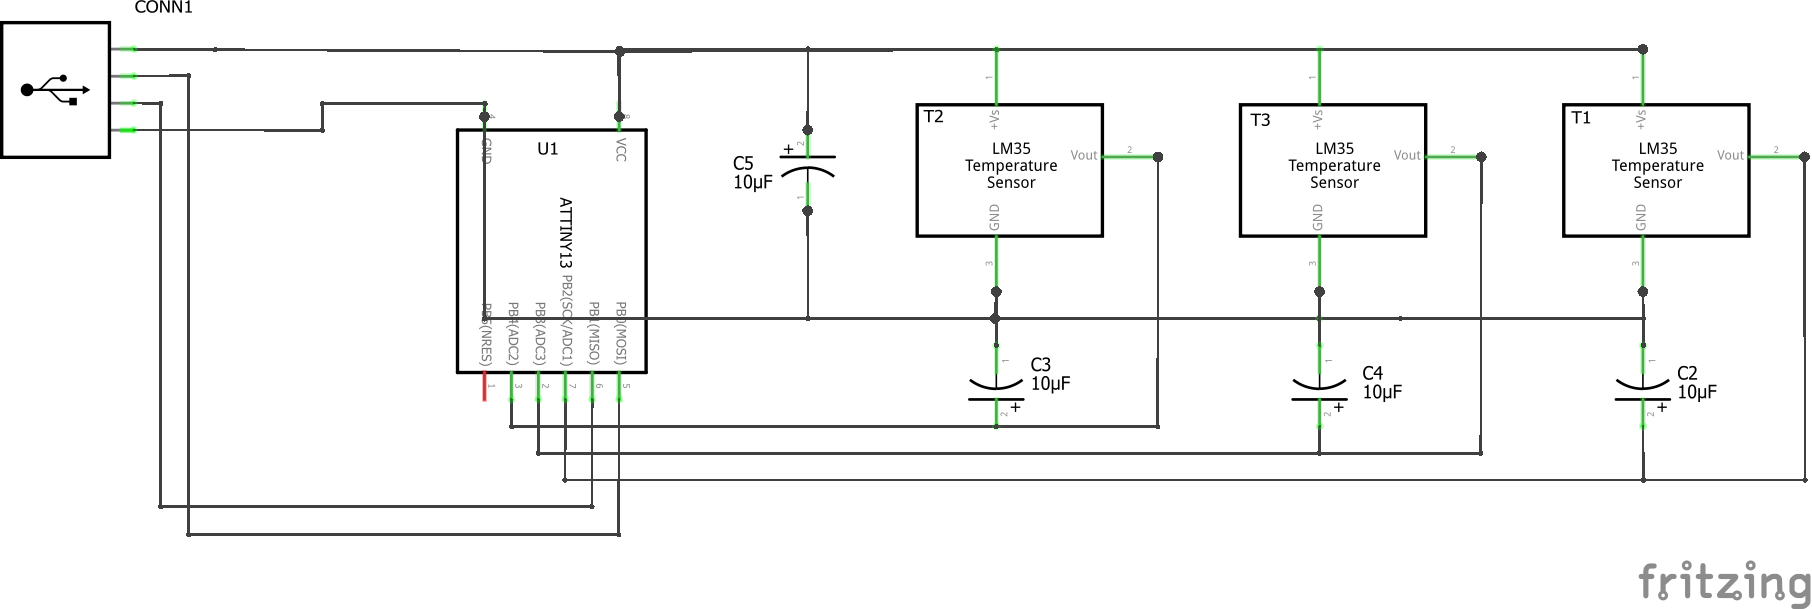
\includegraphics[width=\linewidth]{Figures/Sketch_schem}
			\caption{Conexi\'on al microcontrolador.}
			\label{fig: circuito}
		\end{subfigure}
		\begin{subfigure}{0.23\textwidth}
			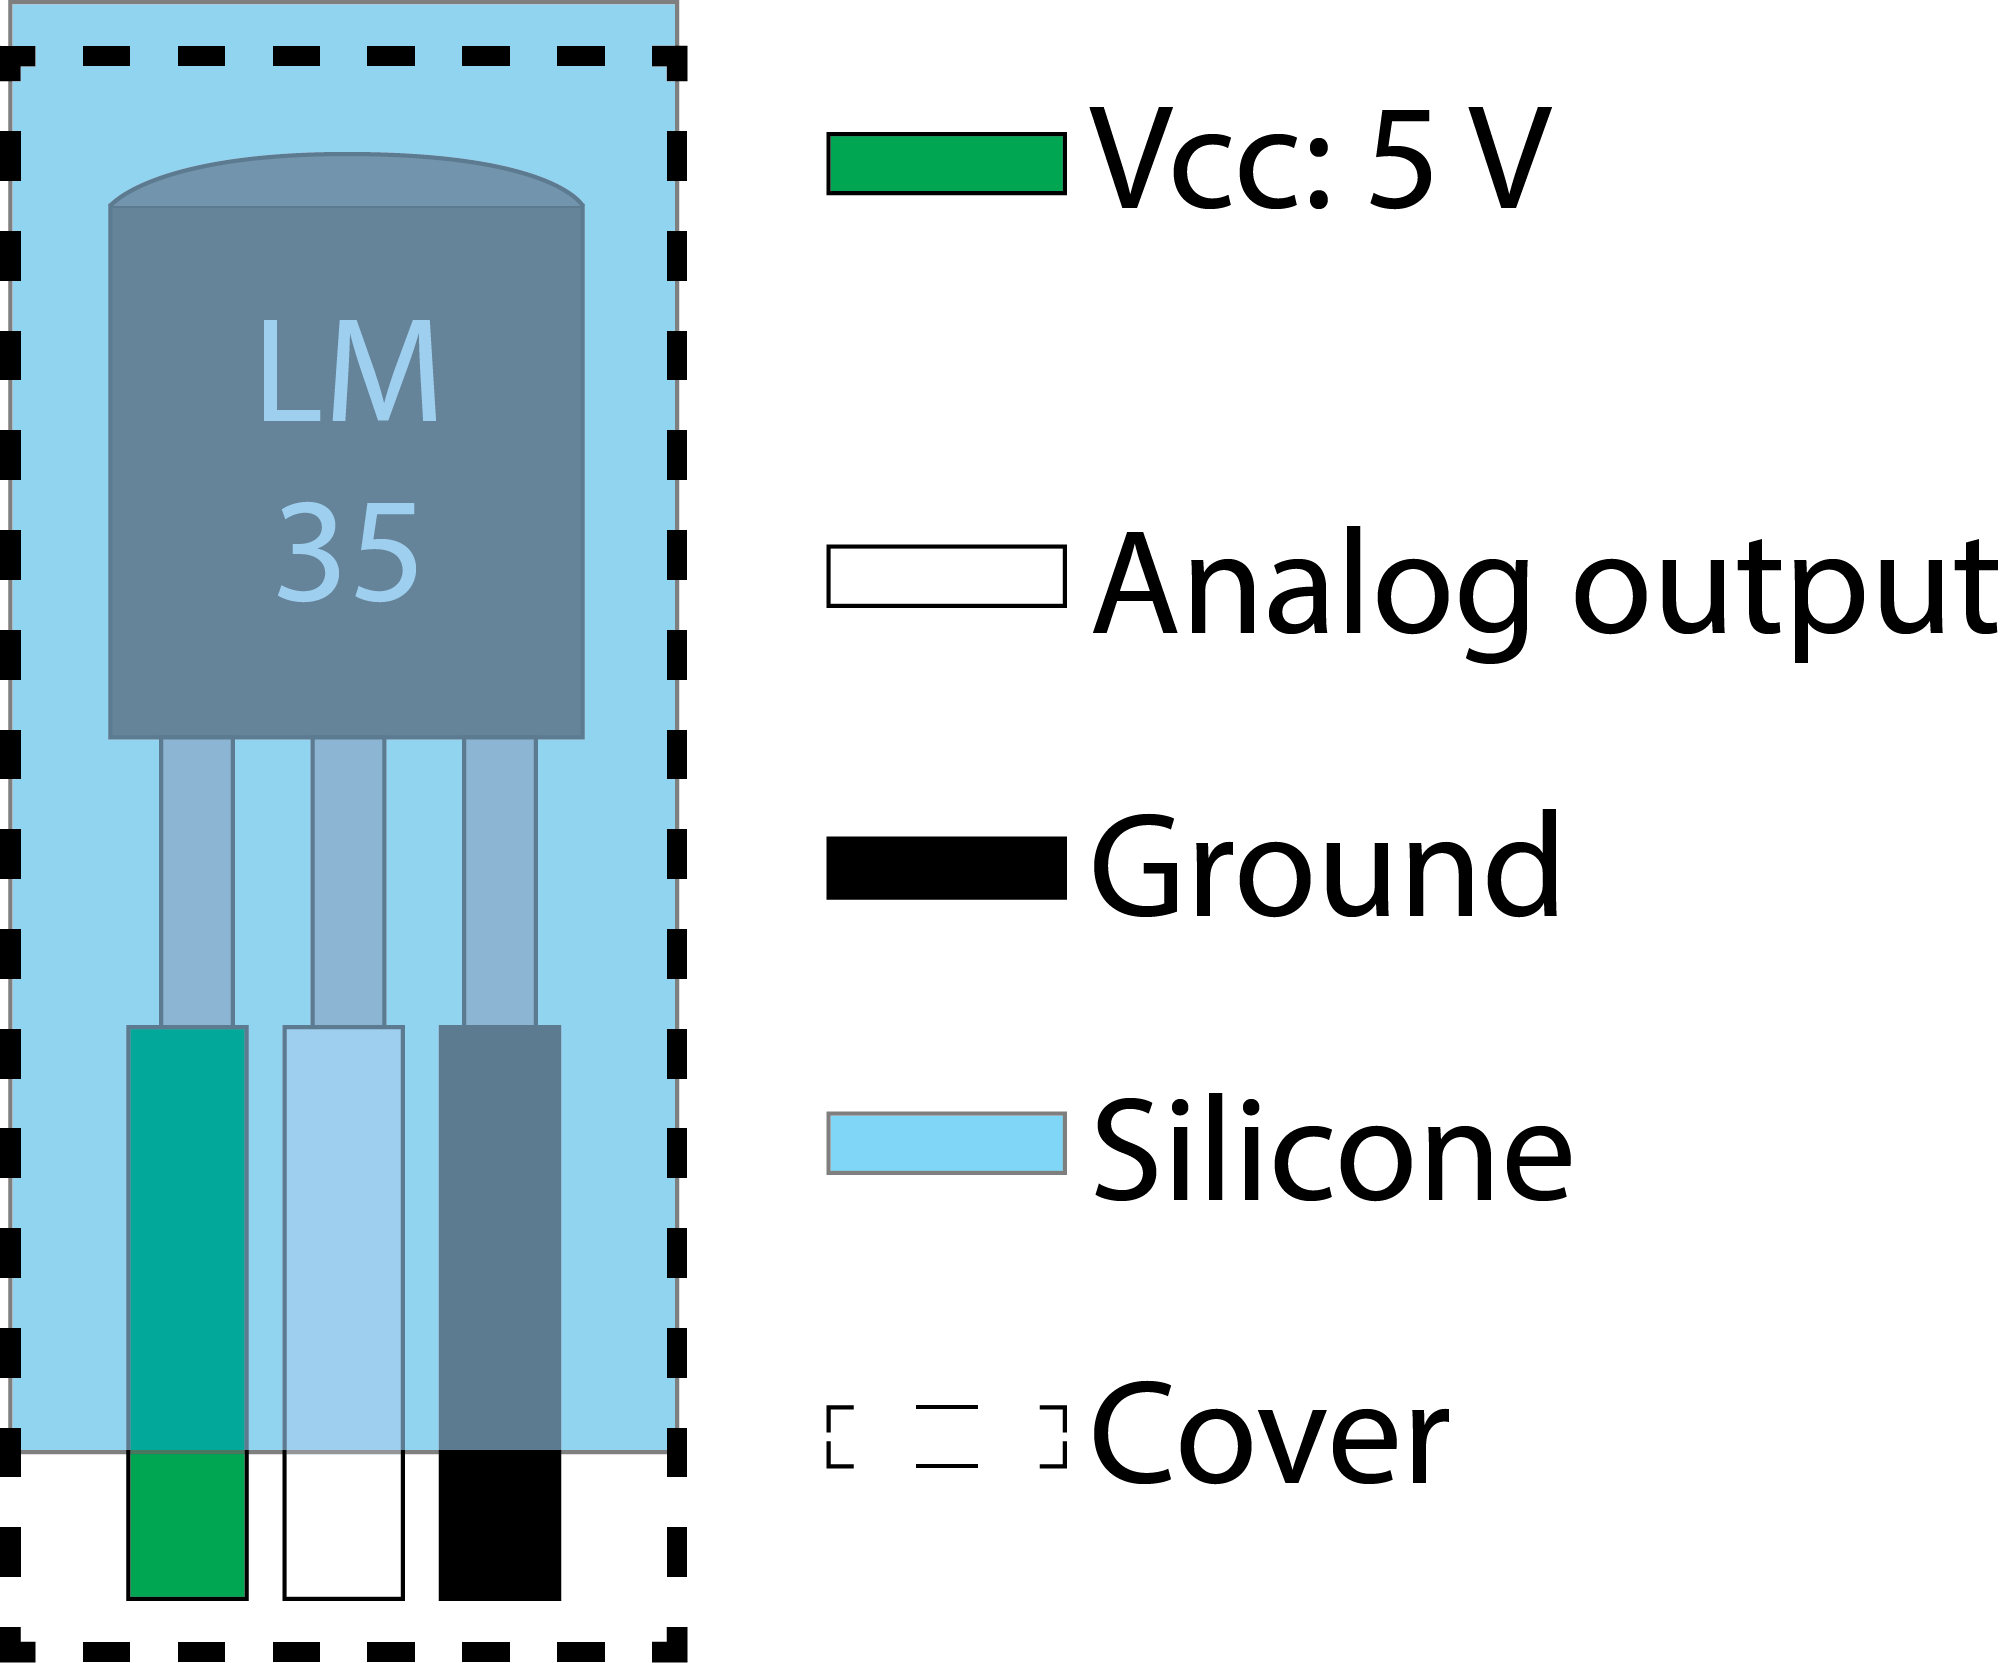
\includegraphics[width=\linewidth]{Figures/Sensor}
			\caption{Cableado del sensor LM35.}	
			\label{fig: sensors}
		\end{subfigure}
		\caption{Circuito del sistema de monitoreo de temperatura.}	
	\end{figure}

	Los sensores, uno para el baño interno, baño externo y temperatura ambiente, a su vez fueron conectados a un microcontrolador ATtiny 13 \cite{attiny13} (\autoref{fig: circuito}), el cual hace las veces de central de procesamiento que unifica las señales de los tres sensores y las envía a un computador usando el protocolo de comunicación UART (\textit{Universal Asynchronous Receiver-Transmitter} por sus siglas en inglés). Para convertir las señales de los sensores a un valor digital se usa el ADC (\textit{Analog to Digital Converter} por sus siglas en inglés) con el que cuenta el microcontrolador. El ADC compara el voltaje de la señal de entrada con un valor de referencia de voltaje y determina que fracción de voltaje corresponde la señal de entrada, este valor relativo ($k$) se encuentra entre 0 y 2$^{n}$ ($n$ es el número de bits del ADC), donde 0 implica un valor igual al de la tierra del circuito, y 2$^n$ tiene lugar cuando la señal de entrada tiene el mismo valor que el voltaje de referencia, los valores intermedios son lineales con los límites, de tal forma que es posible reconstruir el valor de la señal en voltios mediante la siguiente ecuación:
	\begin{equation}
		V = \left(\dfrac{k}{2^n}\right)V_{\text{ref}}
	\end{equation}
	
	En el caso del ATtiny 13, se cuenta con 10 bits en el ADC con cuatro canales, tres de los cuales son usados para los sensores. Como voltaje de referencia se usa un regulador interno del microcontrolador cuyo valor es 1,1 V \cite{attiny13}. Un voltaje de salida del sensor de 1,1 V en el sensor es cercano a 110 \grad{} y 0,0 V cercano a 0 \grad{} pues el fabricante asegura que por cada grado Celsius el voltaje de salida aumenta en 10 mV. El número de bits del ADC permite una resolución cercana a los 0.1 \grad{}, puesto que se tiene que 110 \grad{} pueden ser divididos en $2^{10} = 1024$ niveles distintos. Sin embargo, para lograr una resolución de 0.01 \grad{} se usó una técnica conocida como sobremuestreo \cite{grewal2006oversampling}. Esta técnica tiene sus orígenes en el teorema de Nyquist, el cual establece que para reconstruir una señal es necesario muestrear una señal con el doble de la frecuencia de la frecuencia máxima en la señal \cite{alexander2009fundamentals}. En el caso de la temperatura de los baños de agua y ambiente, se espera que la frecuencia máxima sea relativamente baja, del orden del tiempo de respuesta del sensor el cual es del orden de segundos. En particular se tiene que para $w$ bits adicionales en el ADC es necesario muestrear $4^w$ veces adicionales la señal. Dado que se tiene un rango cercano a los 100 grados y se quiere una resolución de 0,01 \grad{} es necesario diferenciar 10.000 niveles distintos de voltaje, lo cual implica al menos 14 bits ($2^{14}=$16.384), sin embargo, se eligen muestrear 4096 veces con frecuencia de 150 kHz, lo cual equivale a 16 bits en el ADC.
	
	Los sensores fueron calibrados usando el baño externo, y el termómetro de mercurio previamente usado en la verificación de la lectura de temperatura del sensor interno del calorímetro. Para esto se realizó una rampa de calentamiento discreta de 10 \grad{} hasta 50 \grad{} con pasos de 5 \grad{} y tiempos de estabilización de 20 minutos. Se escribió un algoritmo que calcula el valor promedio y desviación estándar de una lectura de voltaje para los intervalos estacionarios de la rampa. Este algoritmo realiza lo siguiente:
	\begin{enumerate}
		\item Para cada instante de tiempo considera el promedio de voltaje de los tres sensores.
		\item Saca el valor absoluto de la derivada de los datos en el tiempo.
		\item Aplica un filtro de medianas con kernel 507 sobre los datos anteriores (líneas continuas rojas en la \autoref{fig: calAlgorithm}).
		\item Los puntos con valores menores a 0,05 se les asigna el valor 0, para los otros valores se asigna 0,5 (lineas segmentadas en la \autoref{fig: calAlgorithm}).
		\item Se considera que los puntos donde el valor anterior corresponde a 0 son estables, sobre estos intervalos calcula el promedio y desviación estándar de cada sensor.
	\end{enumerate}
	
	\begin{figure}[h]
		\centering
		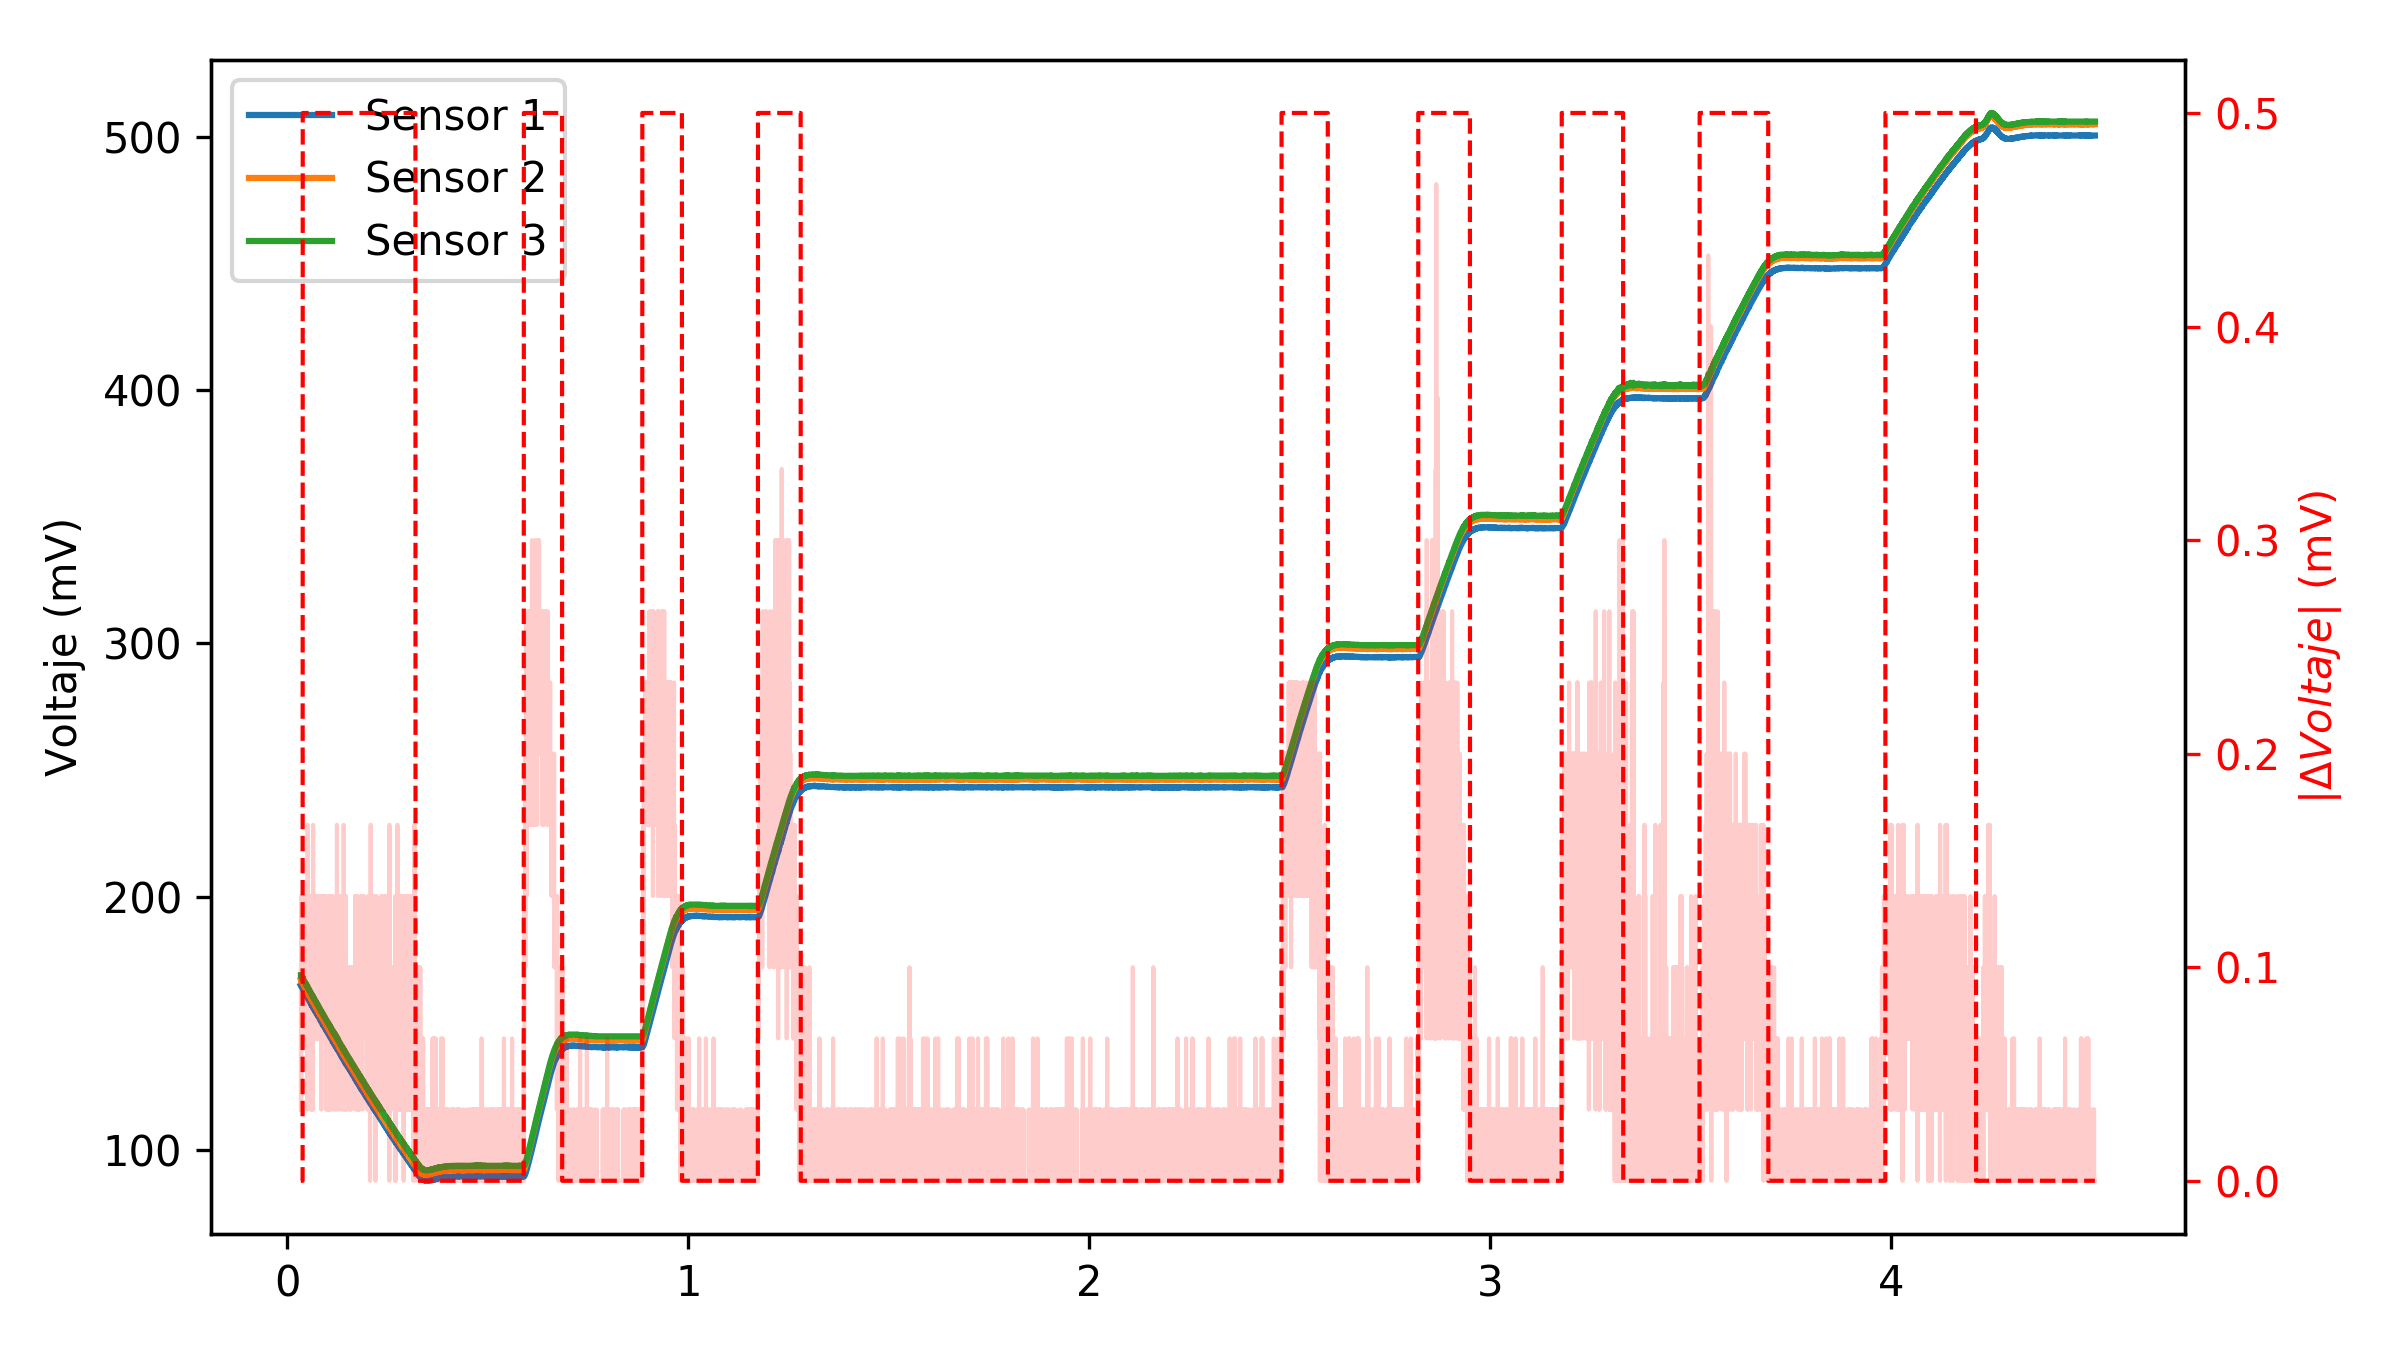
\includegraphics[width=\linewidth]{../Data/TemperatureCalibration/dV-t}
		\caption{Voltajes registrados en la rampa de calentamiento de calibración de los sensores.}
		\label{fig: calAlgorithm}
	\end{figure}

	Los valores de voltaje de los intervalos estacionarios de la rampa fueron relacionados con la temperatura del termómetro de mercurio en la \autoref{fig: voltageTemperature}, en donde se observó una tendencia lineal, cuya pendiente es cercana a 10 mV, lo cual concuerda con lo reportado por el fabricante \cite{instruments1999lm35}. A partir de las relaciones obtenidas con la regresión lineal, se reconstruyó la \autoref{fig: calAlgorithm} en función de la temperatura.
	\begin{figure}[h]
		\centering
		\begin{subfigure}{0.45\linewidth}
			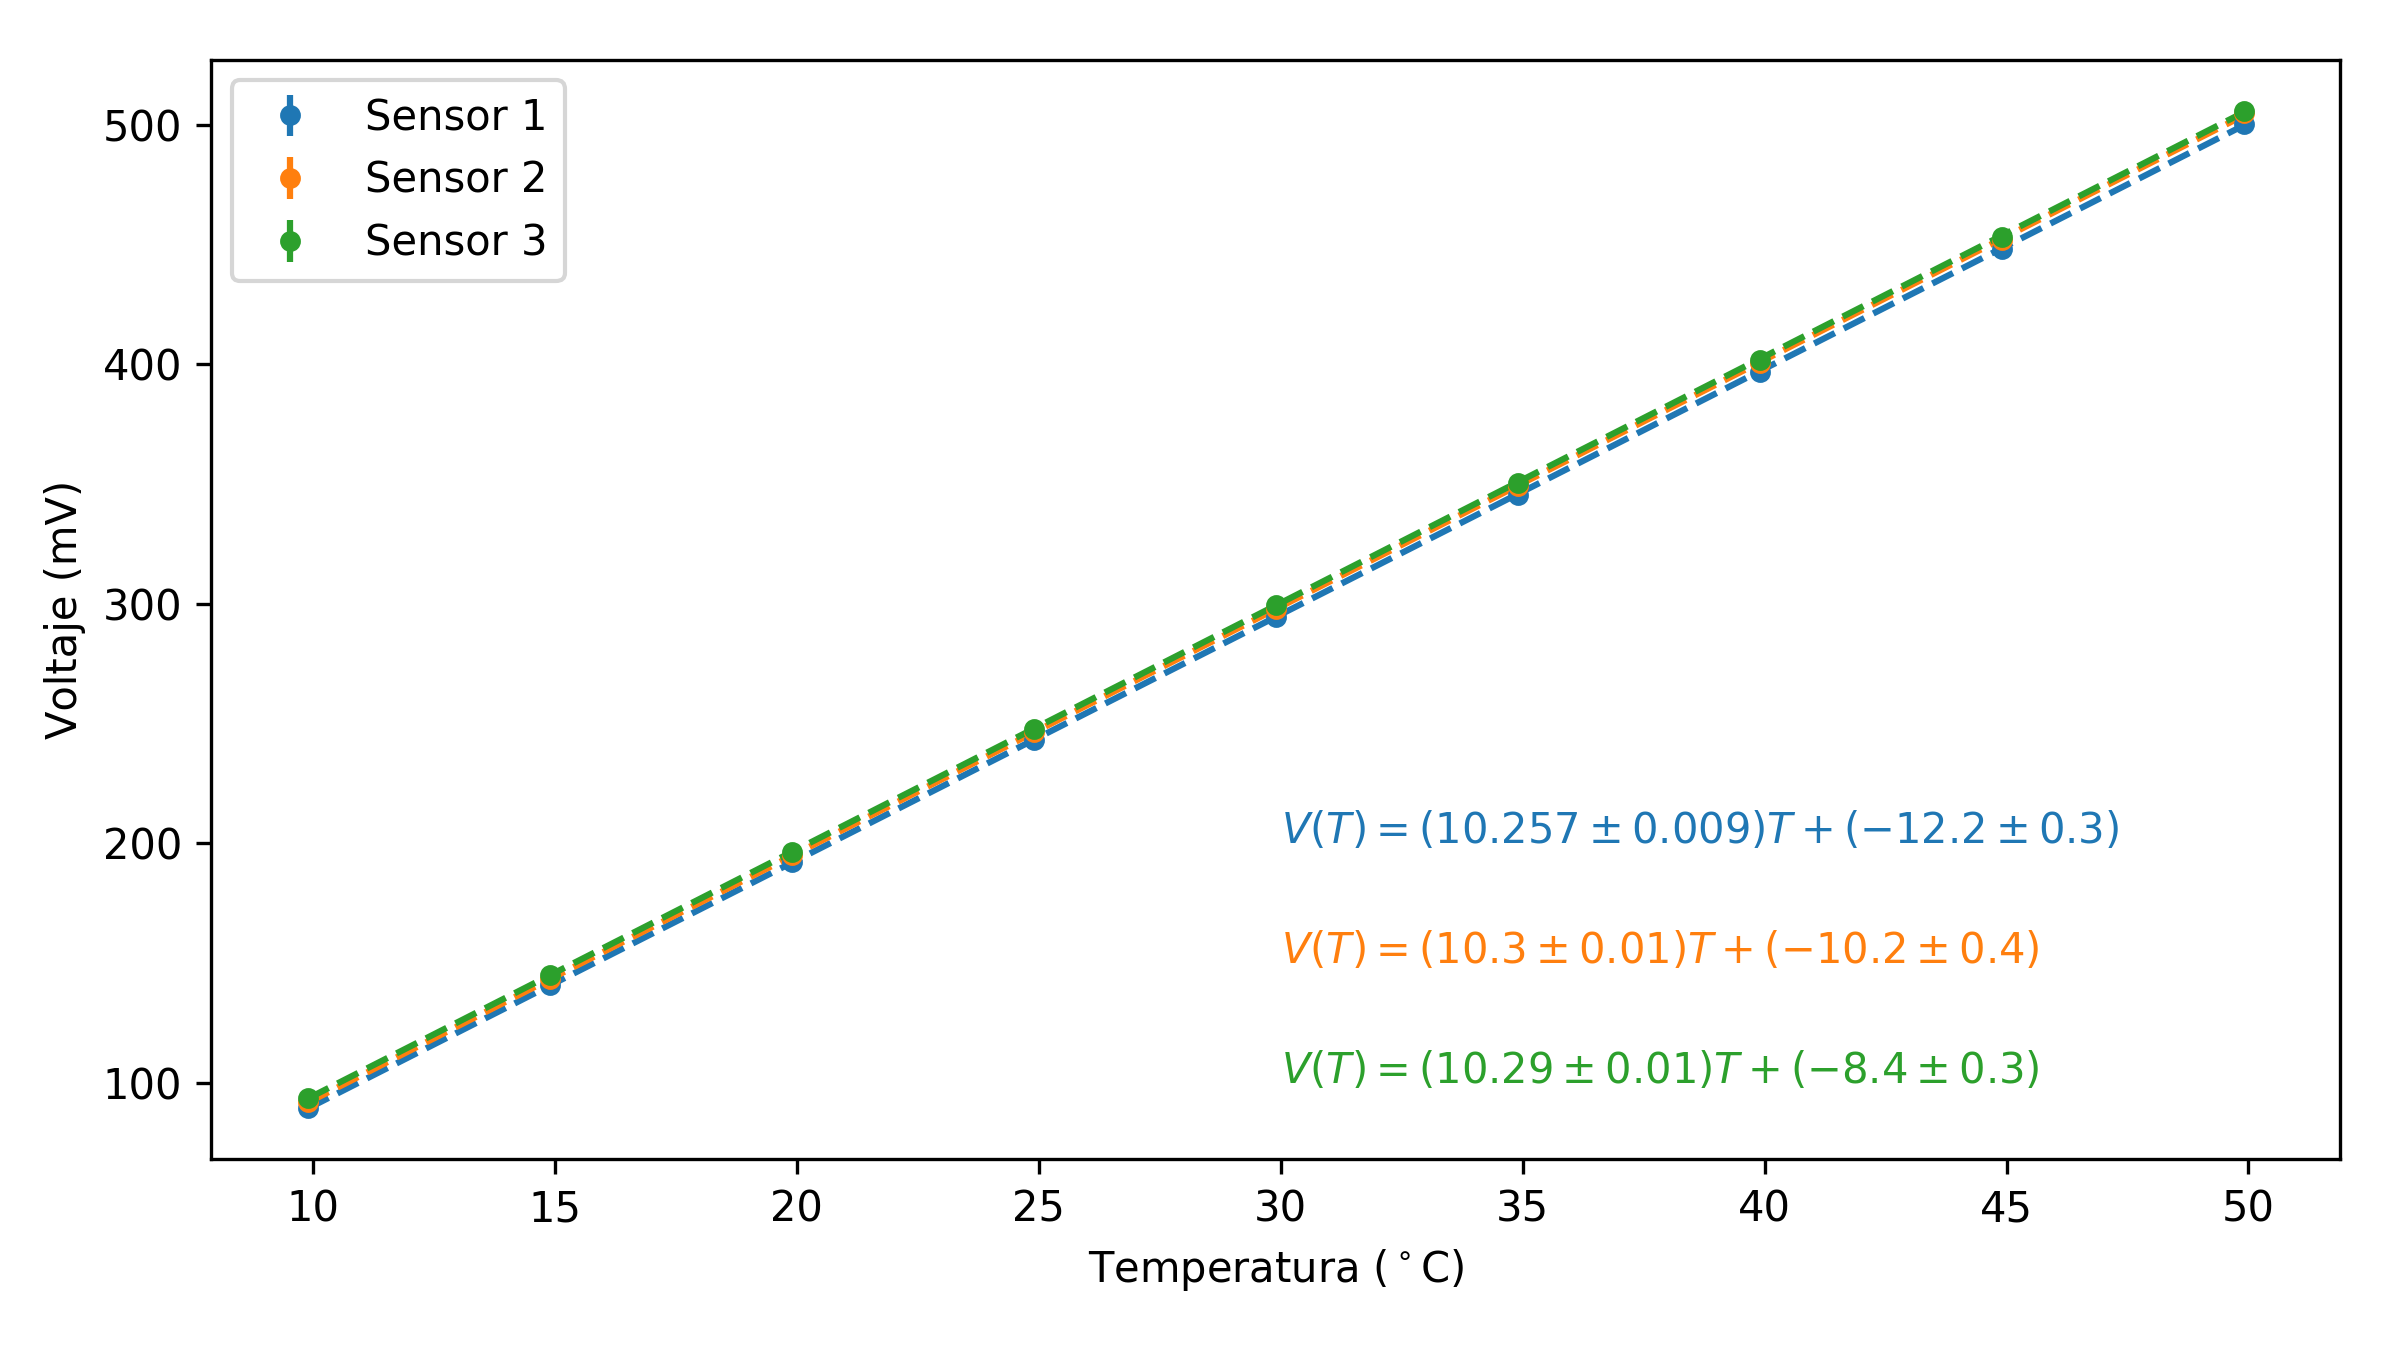
\includegraphics[width=\linewidth]{../Data/TemperatureCalibration/V-T}
			\caption{Voltajes registrados en la rampa de calentamiento de calibración de los sensores.}
		\end{subfigure}
		\begin{subfigure}{0.45\linewidth}
			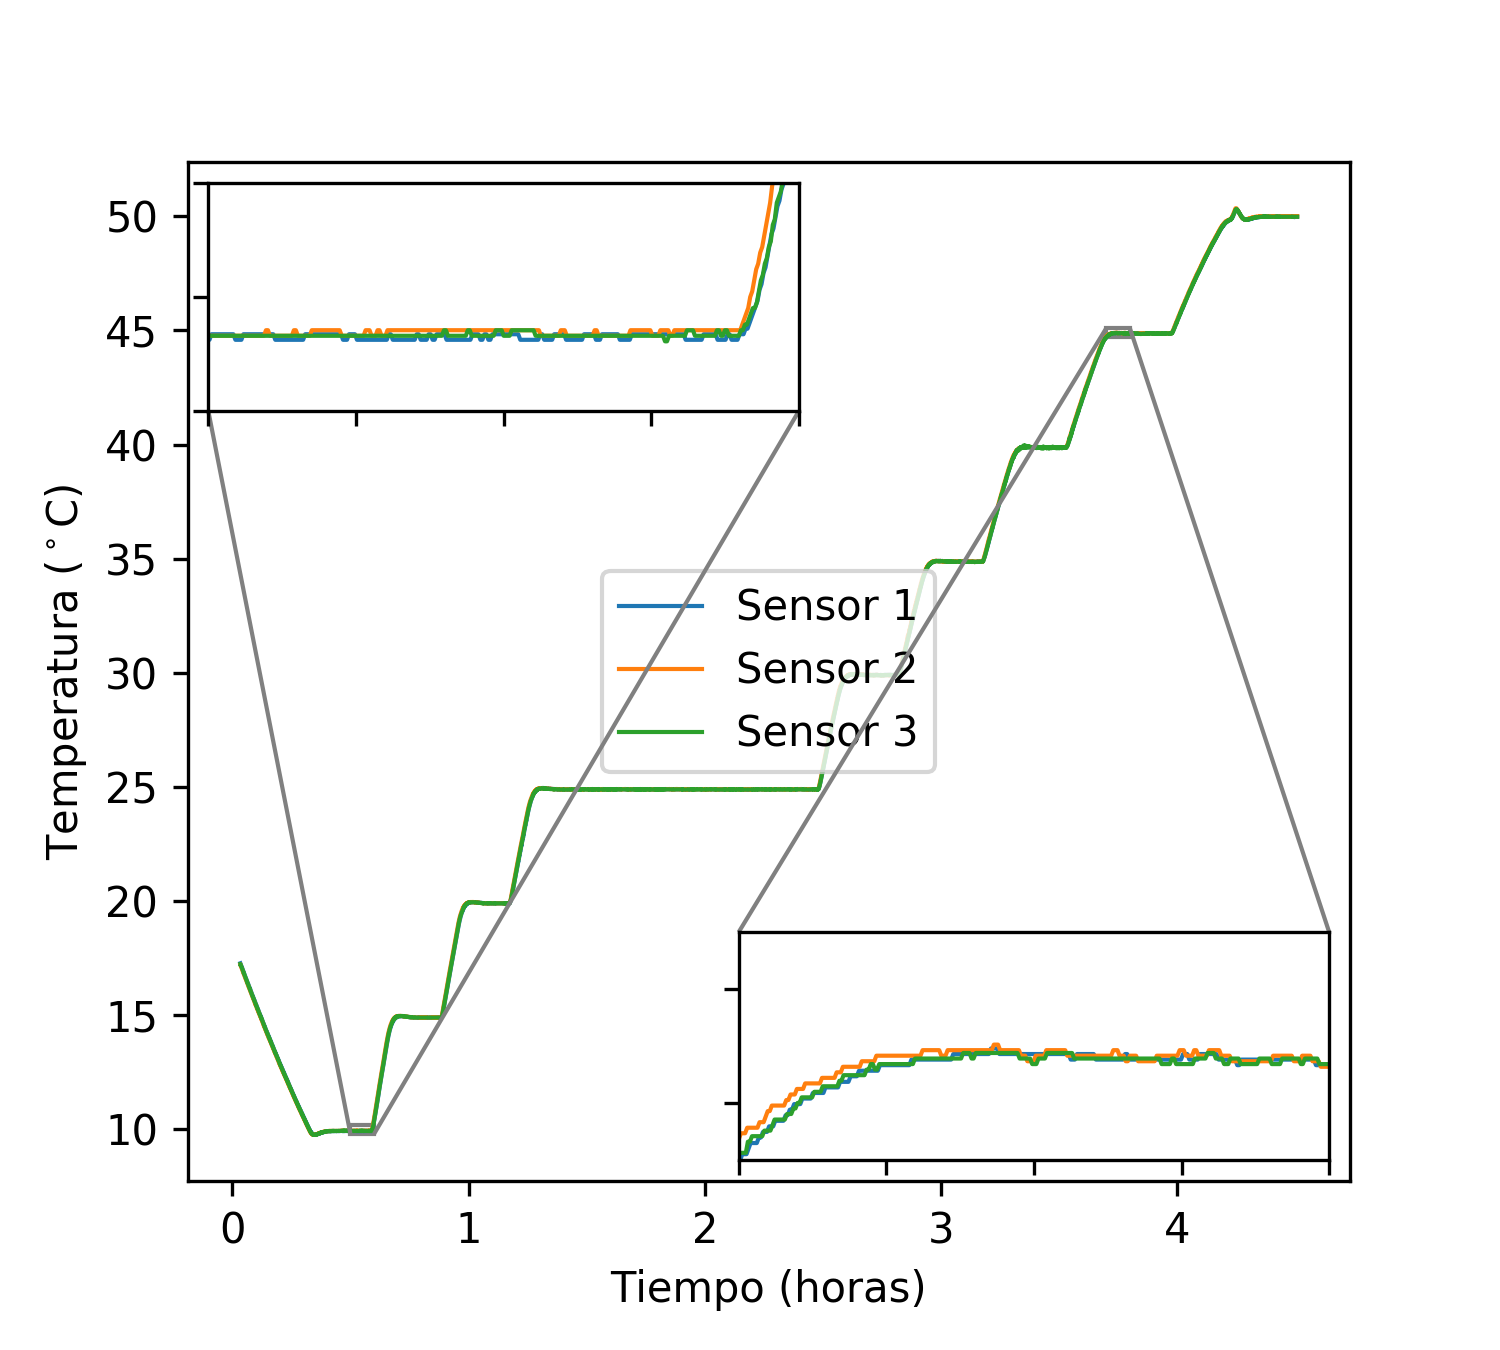
\includegraphics[width=\linewidth]{../Data/TemperatureCalibration/T-t}
			\caption{Voltajes registrados en la rampa de calentamiento de calibración de los sensores.}
		\end{subfigure}
		\caption{Resultados de la calibración del sistema de monitoreo de la temperatura.}
		\label{fig: voltageTemperature}
	\end{figure}
	\pagebreak

	Una vez calibrados los sensores, se escribió un programa en Python para facilitar la visualización de los datos en tiempo real, cuyo código se encuentra en la \autoref{anx: interfaz}. Además, para introducir el sensor usado en el baño interno del calorímetro sin que este estuviera expuesto directamente a la temperatura ambiente, se imprimió una tapa en 3D con un filamento de PLA (ácido poliláctico) para usar uno de los espacios reservados para un cilindro de medición del calorímetro.
	\begin{figure}[h]
		\centering
		\begin{subfigure}{0.45\linewidth}
			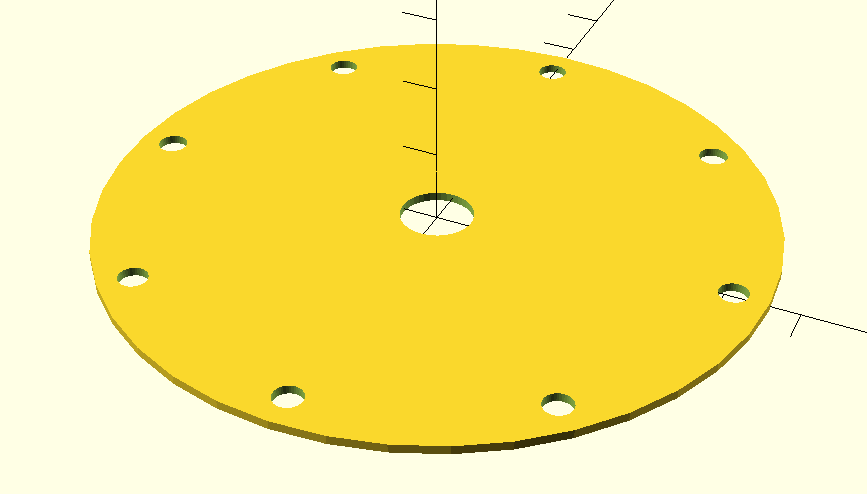
\includegraphics[width=\linewidth]{Figures/PLAdisk}
			\caption{Disco impreso para facilitar el acceso del sensor al baño térmico del calorímetro.}
		\end{subfigure}
		\begin{subfigure}{0.45\linewidth}
			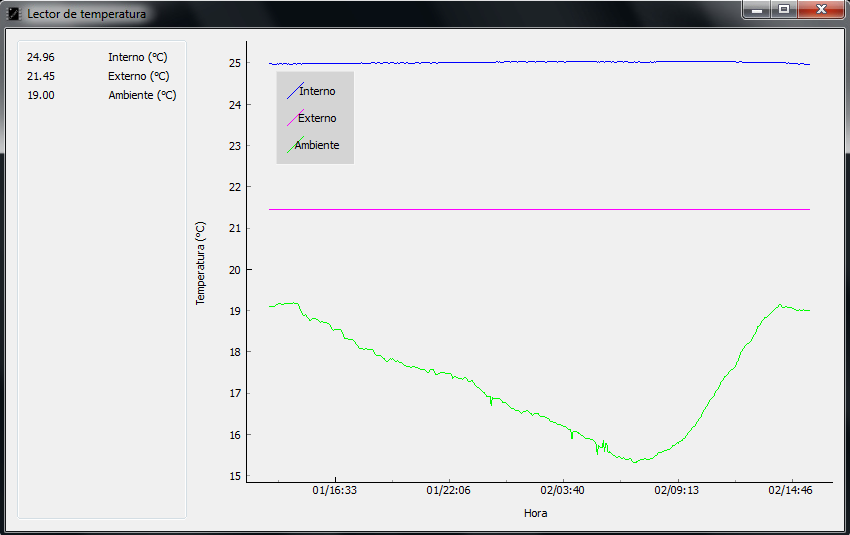
\includegraphics[width=\linewidth]{Figures/temperatureReader}
			\caption{Interfaz gráfica para el monitoreo de la temperatura en tiempo real.}
		\end{subfigure}
		\caption{Accesorios para el sistema de monitoreo de temperatura.}
	\end{figure}

	Con el monitoreo de temperatura establecido fue posible determinar el efecto del baño térmico externo sobre la temperatura del calorímetro. Por ejemplo, para el caso de las oscilaciones que se muestran en la \autoref{tb: temperatureRegister}, se encuentran relacionadas con la temperatura del baño externo, para el caso de temperaturas muy bajas del baño externo se observa que la temperatura del baño interno se encuentra estable, sin embargo los calefactores se encuentran trabajando fuera del rango completamente prendidos, y a temperaturas del baño externo intermedias, la temperatura del baño interno oscila. Esto se puede entender si se considera que los sistemas térmicos presentan inercia, por lo cual mientras el sensor de temperatura registra una temperatura menor a la deseada, aplicará sobre los calentadores potencia, una vez se sobre pase este valor los calentadores se apagarán pero el agua de los alrededores se continuará calentando por algún tiempo, posteriormente el sistema detectará que la temperatura ha disminuído prendiendo nuevamente los calentadores haciendo que la temperatura en general oscile como se muestra en la \autoref{fig: temperatureRipple}.
	\begin{figure}[h]
		\centering
		\begin{subfigure}{0.49\linewidth}
			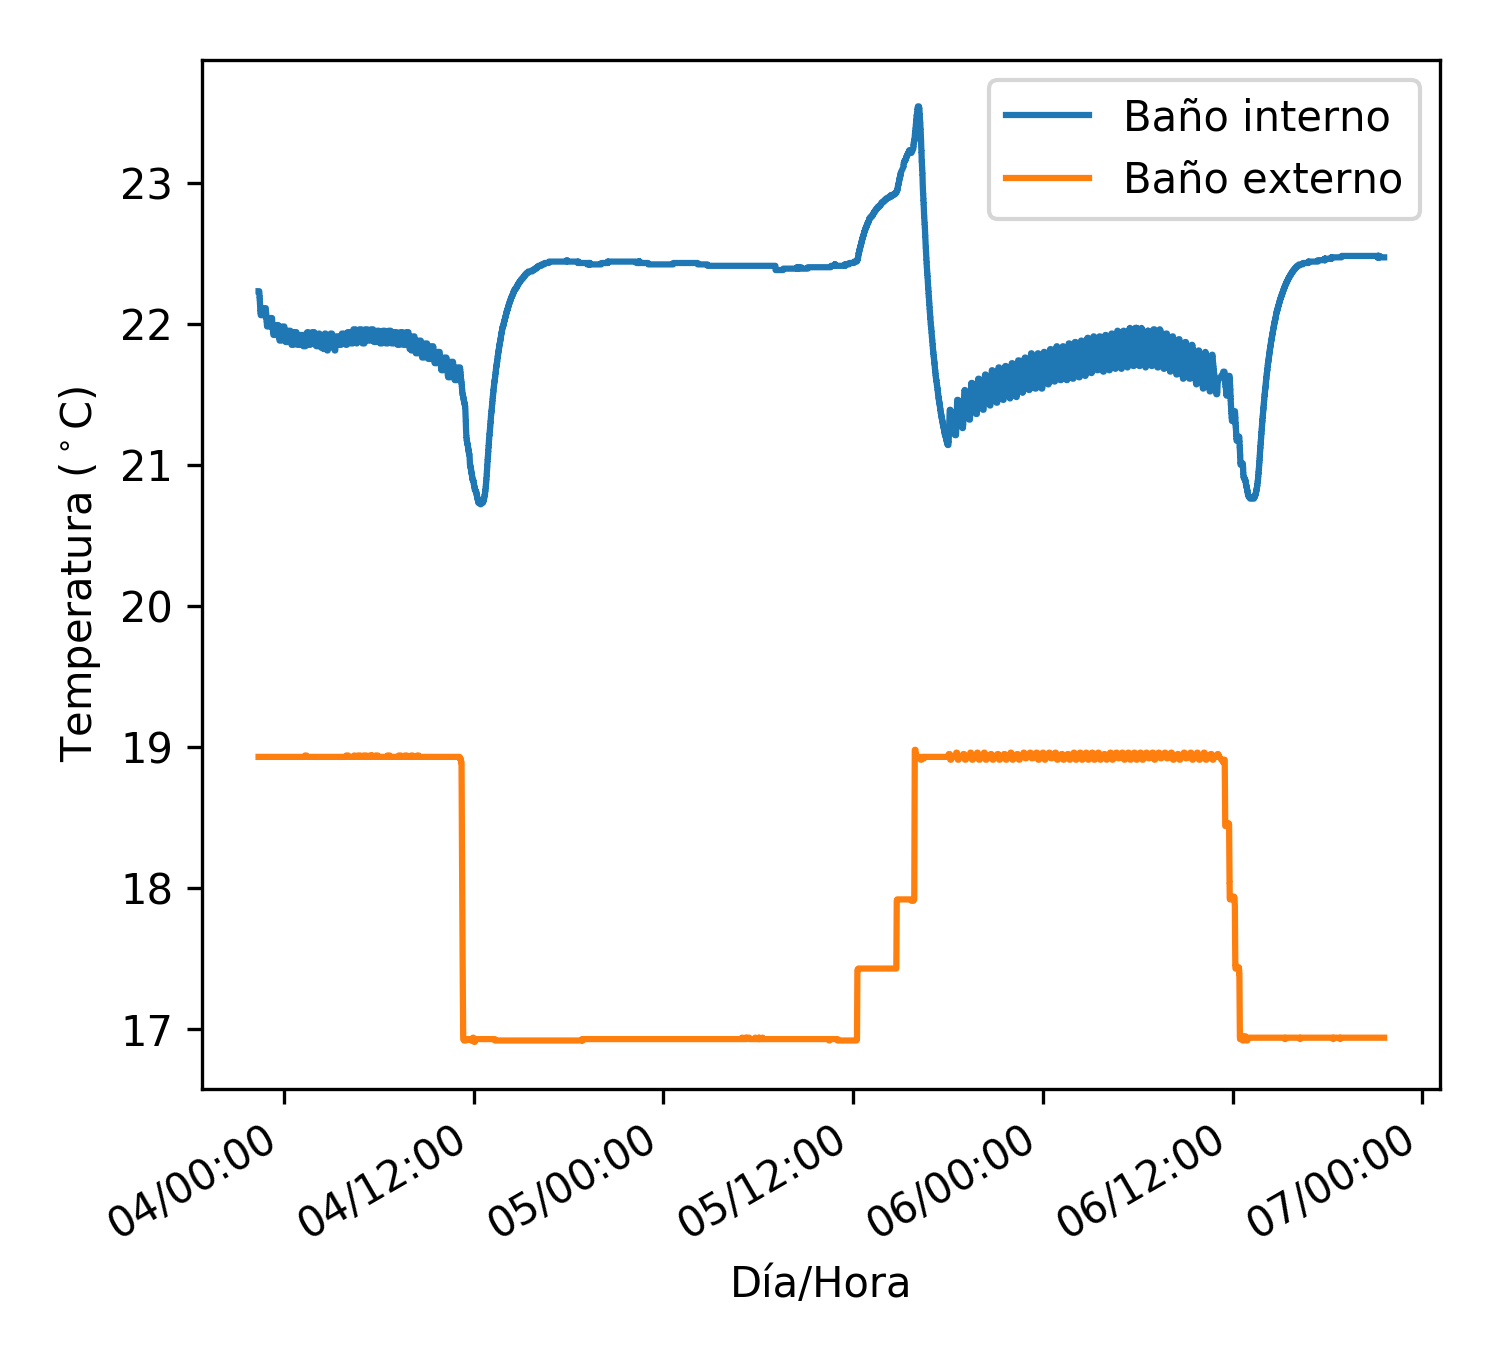
\includegraphics[width=\linewidth]{../Data/TemperatureStability/temperatureRipple}
			\caption{Oscilaciones debidas a una temperatura del baño externo intermedia.}
			\label{fig: temperatureRipple}
		\end{subfigure}
		\begin{subfigure}{0.49\linewidth}
			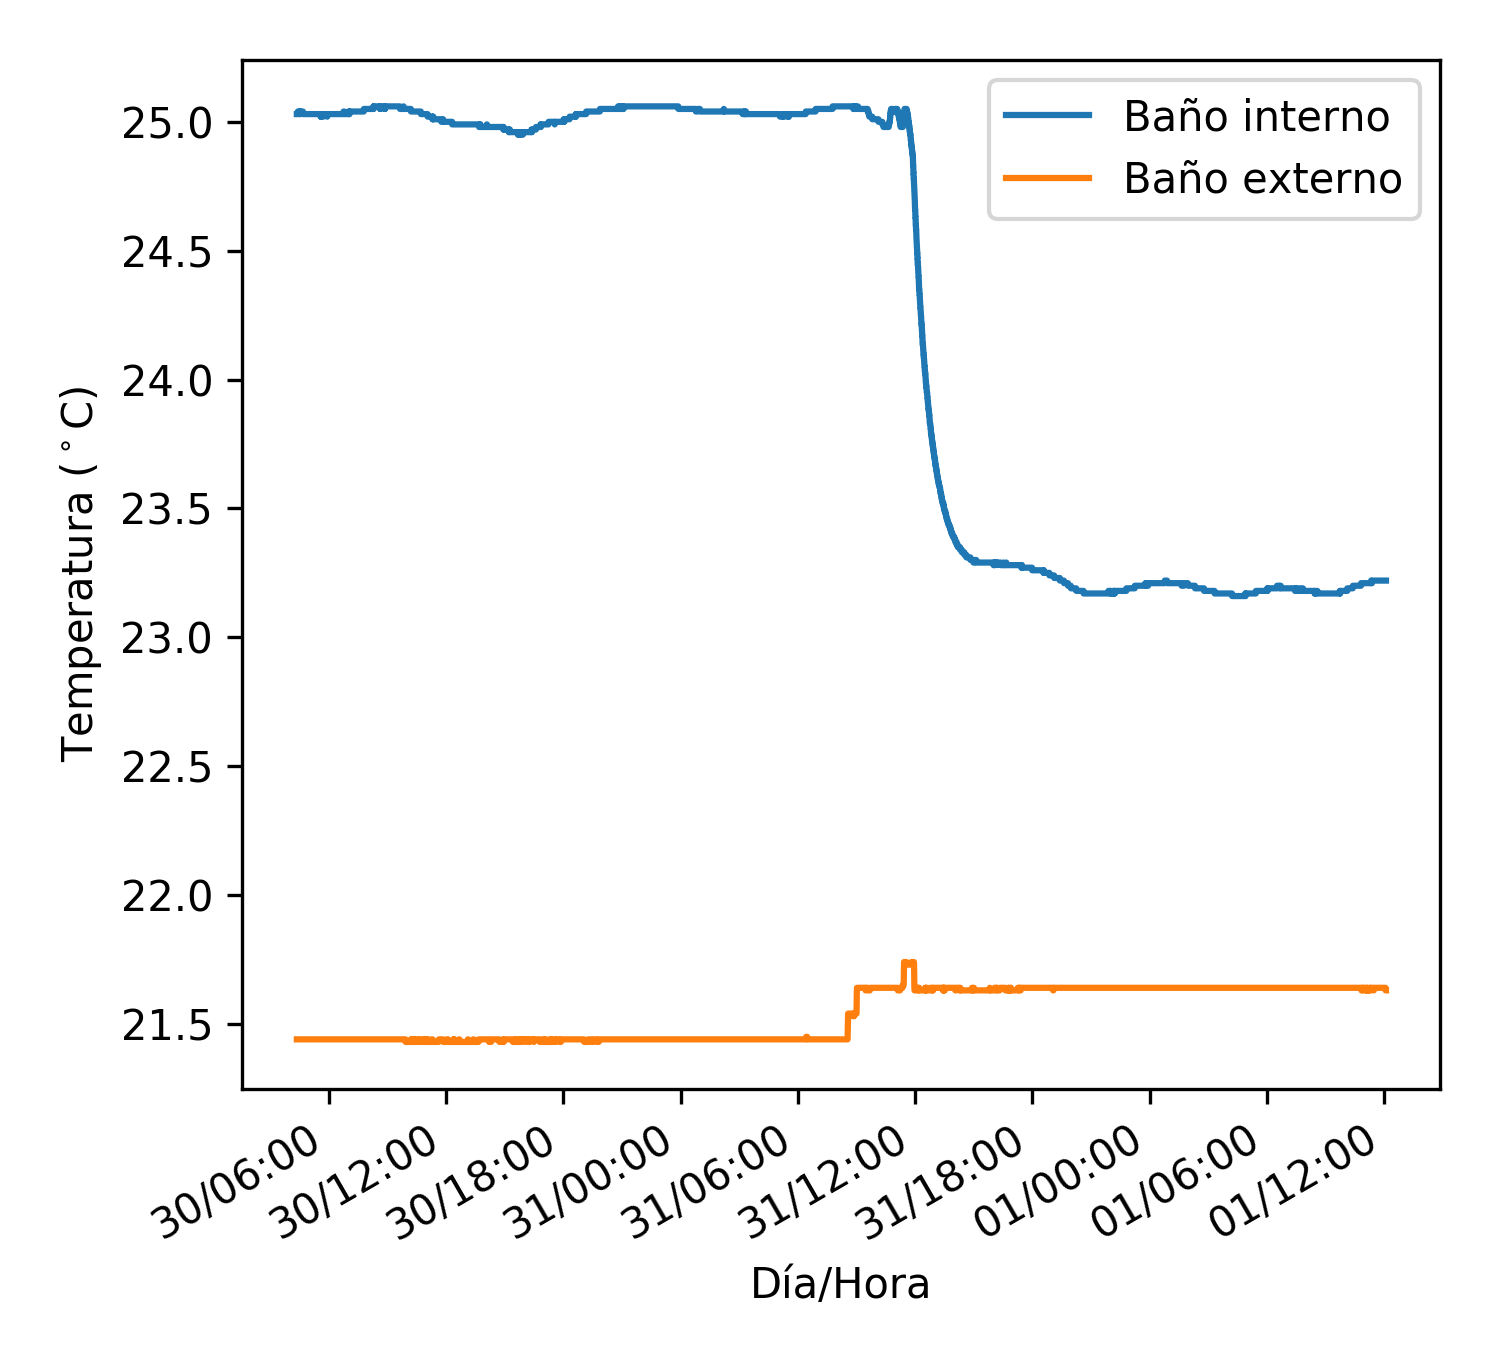
\includegraphics[width=\linewidth]{../Data/TemperatureStability/temperatureSensibility}
			\caption{Caída de la temperatura del baño interno debido al aumento de 0,20 \grad{} en el baño externo.}
			\label{fig: temperatureSensibility}
		\end{subfigure}
		\caption{Efecto de la temperatura del baño externo sobre la temperatura del baño interno.}
		\label{fig: externalEffects}
	\end{figure}

	En la \autoref{fig: temperatureSensibility} se observa cómo la temperatura del calorímetro puede variar bruscamente cuando los calentadores trabajan fuera de rango. En el caso de esta figura, la temperatura del calorímetro se encontraba estable, el calentador fino siempre en el rango de trabajo, mientras que el precalentador ocasionalmente salía del rango de trabajo, sin embargo, al aumentar la temperatura del baño 0,20 \grad{} el equipo disminuyó su temperatura y no volvió aumentar. 
	
	En general la \autoref{fig: externalEffects} muestra la dificultad de estabilizar el equipo a una temperatura determinada, puesto que se debe encontrar la pareja correcta de valores en las resistencias de décadas, junto con la temperatura del baño externo, siendo los dos particularmente sensibles al valor del otro. Pues como fue mencionado anteriormente, aunque en la \autoref{fig: temperatureSensibility} el sistema parezca estable, los calentadores internos están funcionando fuera del rango.
	
	Finalmente, se logró determinar la configuración en donde los calentadores se encuentran en el rango de trabajo y el equipo es estable a $25.02 \pm 0.03$ \grad{}, esta configuración se muestra en la \autoref{tb: decadeResistorsAfter}. Además, el sensor de temperatura ambiente, probó ser útil, pues la pequeña variación en la temperatura interna del calorímetro se encuentra correlacionada con la temperatura ambiente, pues en la \autoref{fig: temperatureResults} se observa que los máximos de temperatura interna ocurren en los mínimos de temperatura ambiente.
	\begin{table}[h]
		\centering
		\caption{Valores de las resistencias de década, para una temperatura de 25 \grad{}, obtenida en octubre.}
		\begin{tabular}{r|cccc|l}
			\hline
			\textbf{Baño interno (\grad{})} & A ($10^4$ $\Omega$) & B ($10^3$ $\Omega$) & C ($10^2$ $\Omega$) & D ($10^1$ $\Omega$) & \textbf{Baño externo (\grad{})} \\
			\hline
			$25.02 \pm 0.03$ & 3 & 3 & 6 & 5 & 21,5 \\
			\hline
		\end{tabular}
		\label{tb: decadeResistorsAfter}
	\end{table}

	\begin{figure}[h]
		\centering
		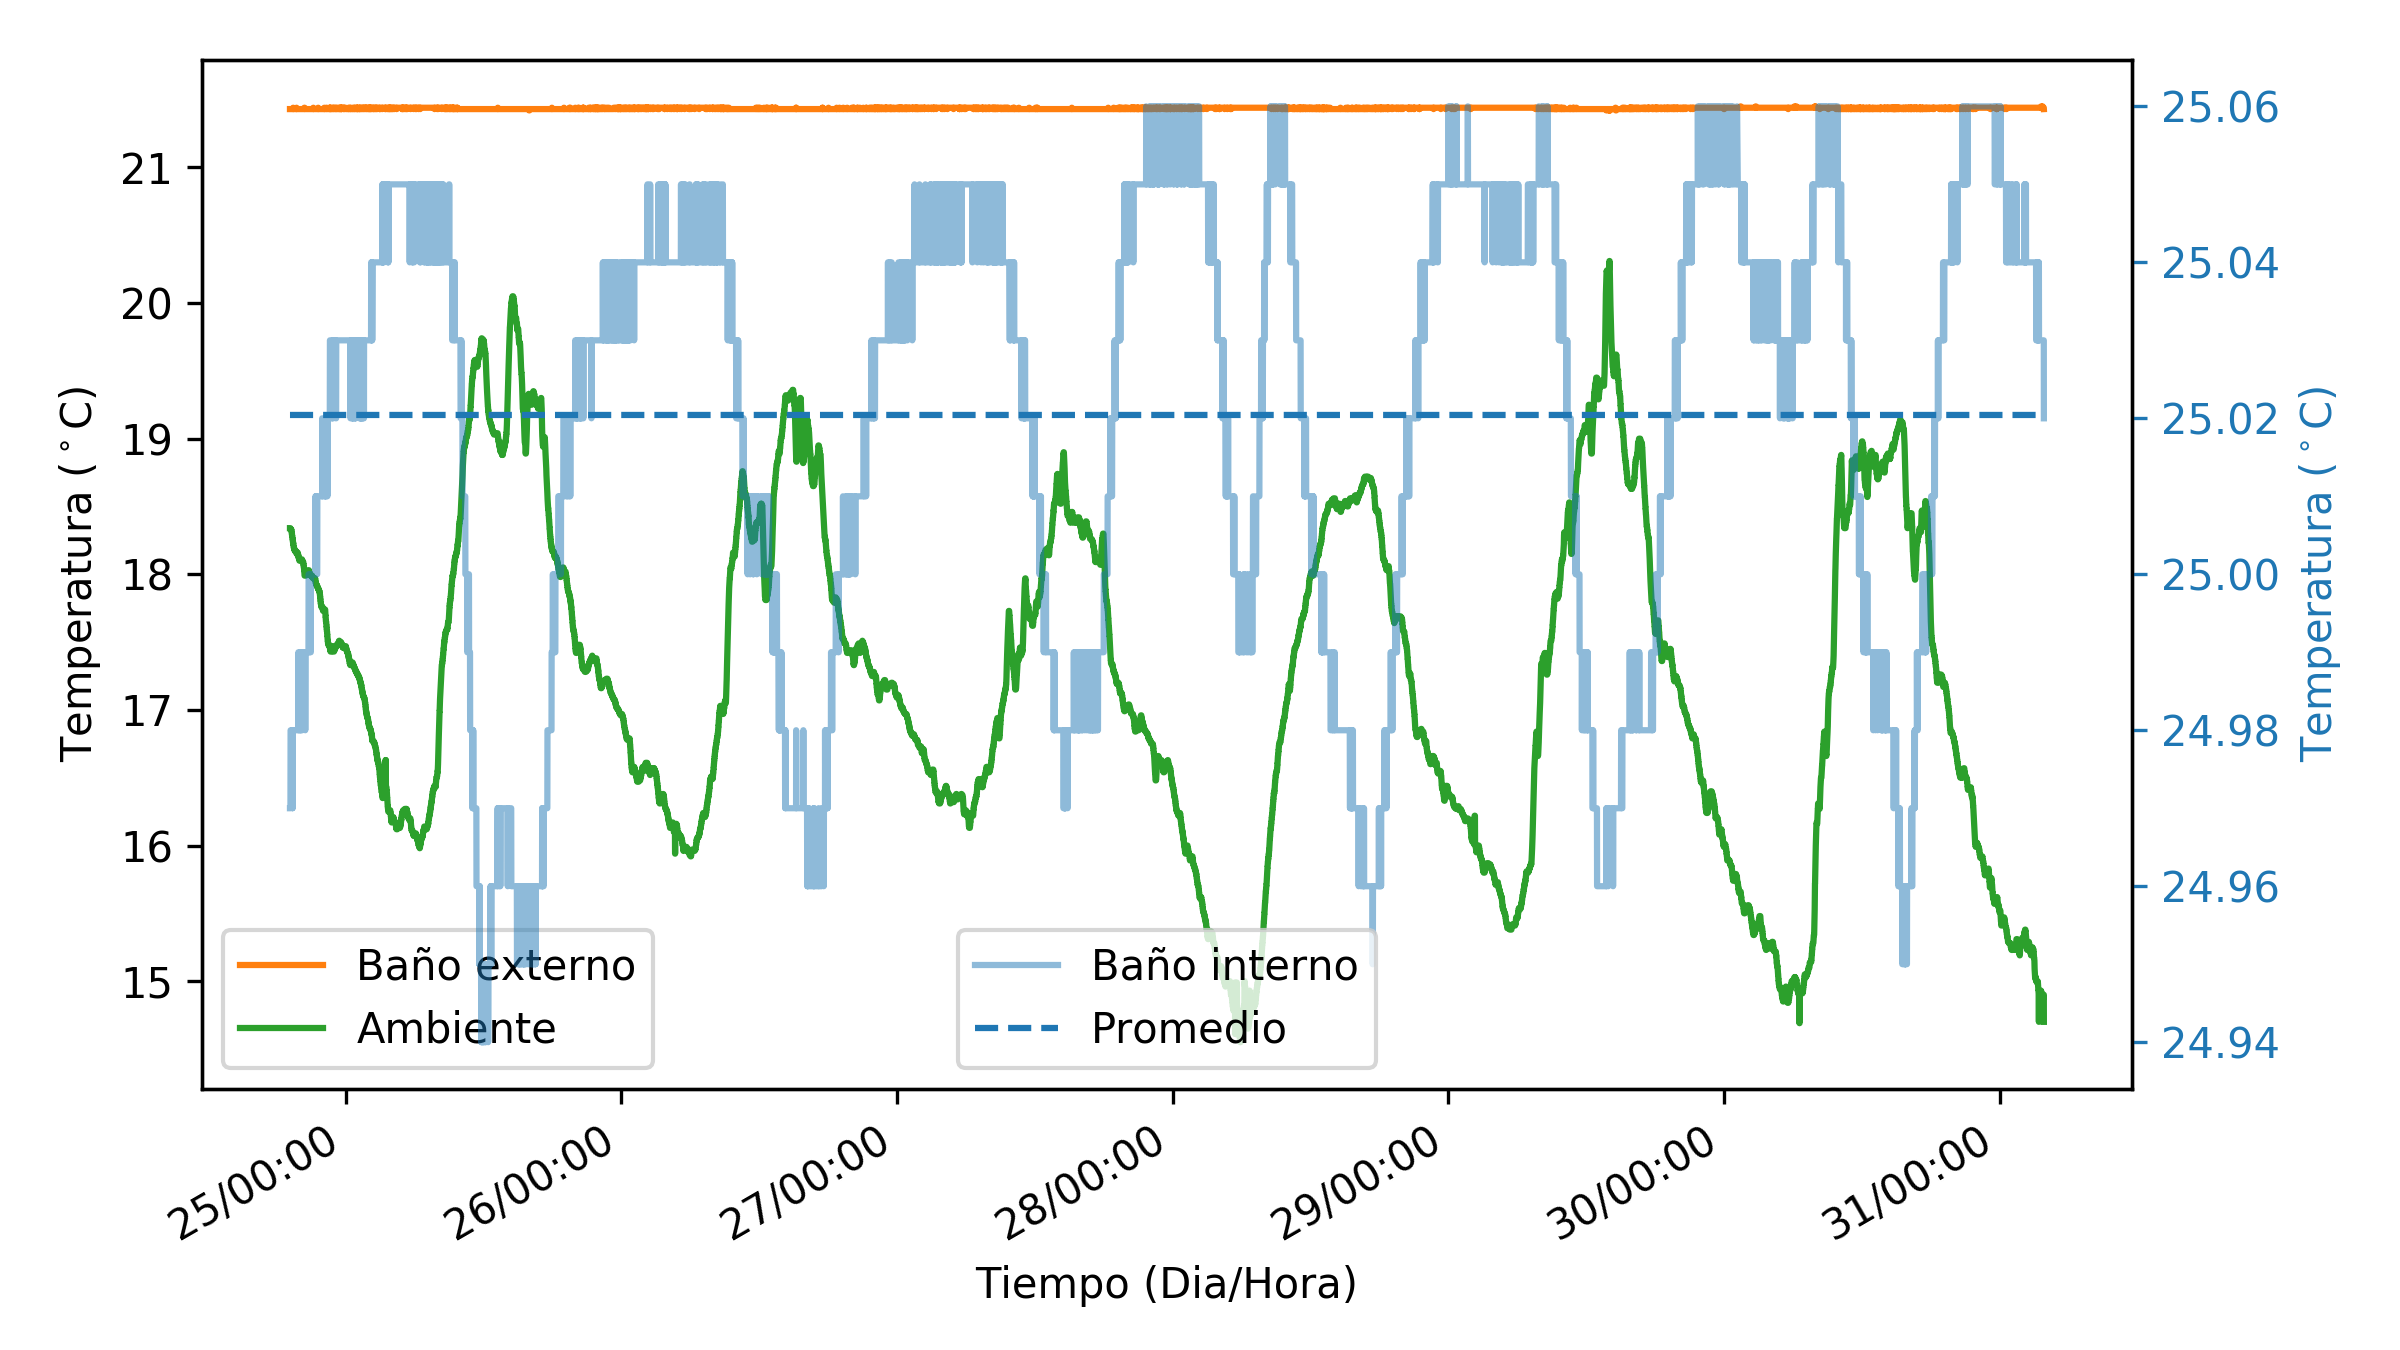
\includegraphics[width=\linewidth]{../Data/TemperatureStability/temperatureStability}
		\caption{Efecto de la temperatura del baño externo sobre la temperatura del baño interno.}
		\label{fig: temperatureResults}
	\end{figure}